\documentclass[11pt]{article}

\usepackage[utf8]{inputenc}
\usepackage[T1]{fontenc}
\usepackage[spanish]{babel}
\usepackage{lmodern}
\usepackage{amsmath,amssymb,amsfonts,mathtools}
\usepackage[a4paper,margin=2.5cm]{geometry}
\usepackage{graphicx}
\usepackage{svg}
\usepackage{xcolor}
\usepackage{hyperref}

\hypersetup{
    colorlinks=true,
    linkcolor=red,
    citecolor=red,
    urlcolor=red
}

% Las ecuaciones se numeran normalmente en negro. En las citas a ecuaciones,
% se conserva el paréntesis negro y solo el número se muestra en rojo y clickeable.
\renewcommand{\eqref}[1]{(\hyperref[#1]{\textcolor{red}{\ref*{#1}}})}

\spanishdecimal{.}
\setlength{\parindent}{0pt}
\setlength{\parskip}{0.45em}
\setlength{\abovedisplayskip}{6pt}
\setlength{\belowdisplayskip}{6pt}
\setlength{\abovedisplayshortskip}{4pt}
\setlength{\belowdisplayshortskip}{4pt}

% Formato de encabezado
\newcommand{\encabezado}[3]{%
{\Large\bfseries #1\par}
\vspace{2pt}
{\normalsize #2\hfill #3\par}
\vspace{6pt}\hrule\vspace{8pt}}

% Comandos auxiliares
\newcommand{\dd}{\,\mathrm{d}}
\newcommand{\ii}{\mathrm{i}}
\newcommand{\e}{\mathrm{e}}
\newcommand{\sen}{\operatorname{sen}}

\begin{document}

\encabezado{Ecuación de Schrödinger para una partícula cuántica en un pozo esférico infinito}{Física Matemática II}{J.R., G.R.}

Considere una partícula de masa $m$ confinada en una esfera de radio $a$. El estado del sistema está descrito por la función de onda $\Psi(r,\theta,\varphi,t)$, la cual satisface la ecuación de Schrödinger dependiente del tiempo,
\begin{equation}\label{eq:schrodinger}
-\frac{\hbar^2}{2m}\nabla^2\Psi = i\hbar\frac{\partial\Psi}{\partial t},
\end{equation}
sujeta a la condición de contorno $\Psi(a, \theta, \varphi, t) = 0$ y a la condición inicial $\Psi(r,\theta,\varphi,0) = \Psi_0(r,\theta,\varphi)$.

\paragraph{Solución: }
Para resolver este problema, aplicamos el MSV. Buscamos primero soluciones separables de la forma
\begin{equation}\label{eq:ansatz-temporal}
\Psi(r,\theta,\varphi,t) = \psi(r,\theta,\varphi) T(t).
\end{equation}

Al sustituir \eqref{eq:ansatz-temporal} en \eqref{eq:schrodinger} y dividir por $\Psi$, obtenemos la separación de la dependencia temporal:
\[
\frac{1}{T} \frac{dT}{dt} = -\frac{iE}{\hbar},
\]
cuya solución es $T(t) = e^{-iEt/\hbar}$, donde $E$ representa la energía del sistema. La parte espacial satisface la ecuación de Helmholtz:
\begin{equation}\label{eq:helmholtz}
\nabla^2\psi + \gamma\psi = 0, \qquad  \gamma = \frac{2mE}{\hbar^2}.
\end{equation}

En coordenadas esféricas, la ecuación \eqref{eq:helmholtz} se separa proponiendo $\psi(r,\theta,\varphi) = R(r)\Theta(\theta)\Phi(\varphi)$. Las soluciones angulares que son univaluadas y finitas en todo el dominio son los Armónicos Esféricos $Y_l^m(\theta, \varphi)$:
\[
\Theta(\theta)\Phi(\varphi) \propto Y_l^m(\theta, \varphi),
\]
donde $l = 0, 1, 2, \dots$ y $m = -l, \dots, l$.

La ecuación radial resultante de \eqref{eq:helmholtz} es la ecuación esférica de Bessel:
\begin{equation}\label{eq:radial-bessel}
\frac{d}{dr}\left(r^2\frac{dR}{dr}\right) + [\gamma r^2 - l(l+1)]R = 0.
\end{equation}
Si $\gamma>0$, las soluciones generales de \eqref{eq:radial-bessel} son las funciones esféricas de Bessel de primera especie $j_l(\sqrt{\gamma}r)$ y de segunda especie $y_l(\sqrt{\gamma}r)$. Si $\gamma<0$, las soluciones son combinación lineal de las funciones esféricas de Bessel modificadas de primera y segunda especie, $i_l(\sqrt{-\gamma}r)$ y $k_l(\sqrt{-\gamma}r)$ respectivamente.
Dado que la función de onda debe ser finita en el origen ($r=0$), descartamos las funciones de segunda especie. Además, la condición de borde en $r=a$, que requiere $R(a)=0$, descarta las funciones modificadas, ya que no se anulan para argumento finito; la comparación gráfica se muestra en las Figuras~\ref{fig:bessel-ordinarias} y~\ref{fig:bessel-modificadas}. Por lo tanto, $\gamma$ debe ser positivo y las soluciones serán de la forma
\begin{equation}\label{eq:radial-positiva}
R(r) = A_{ln} j_l(\sqrt{\gamma}\,r).
\end{equation}

Al imponer explícitamente la condición de borde en $r=a$ sobre \eqref{eq:radial-positiva}, se obtiene
\begin{equation}\label{eq:condicion-borde-radial}
R(a)=A_{ln}j_l(\sqrt{\gamma}\,a)=0.
\end{equation}
Como buscamos soluciones no triviales, $A_{ln}\neq 0$, por lo que \eqref{eq:condicion-borde-radial} implica
\begin{equation}\label{eq:ceros-bessel}
j_l(\sqrt{\gamma}\,a)=0.
\end{equation}
La condición \eqref{eq:ceros-bessel} muestra que, para satisfacer la condición de borde, $\sqrt{\gamma}a$ debe ser una raíz de la función $j_l$. Esto implica que
\begin{equation}\label{eq:gamma-ln}
\sqrt{\gamma_{l,n}} = \frac{\bar\alpha_{l,n}}{a}, \qquad n = 1, 2, 3, \dots
\end{equation}
Consecuentemente, usando \eqref{eq:gamma-ln} en la definición de $\gamma$ dada en \eqref{eq:helmholtz}, la energía del sistema está cuantizada y es dada por
\begin{equation}\label{eq:energia-ln}
E_{l,n} = \frac{\hbar^2 \bar\alpha_{l,n}^2}{2ma^2}.
\end{equation}

La solución general se construye como una superposición de todos los modos separables que satisfacen las condiciones de borde homogéneas, usando la energía cuantizada \eqref{eq:energia-ln}. Por lo tanto,
\begin{equation}\label{eq:solucion-general}
\Psi(r,\theta,\varphi,t) = \sum_{l=0}^{\infty} \sum_{m=-l}^{l} \sum_{n=1}^{\infty} A_{lmn} j_l\left(\frac{\bar\alpha_{l,n} r}{a}\right) Y_l^m(\theta, \varphi) e^{-i E_{l,n} t / \hbar}.
\end{equation}

Para determinar los coeficientes $A_{lmn}$, imponemos la condición inicial. Evaluando \eqref{eq:solucion-general} en $t=0$, se obtiene
\begin{equation}\label{eq:condicion-inicial-descompuesta}
\Psi_0(r,\theta,\varphi)
=
\sum_{l=0}^{\infty} \sum_{m=-l}^{l} \sum_{n=1}^{\infty}
A_{lmn}
 j_l\left(\frac{\bar\alpha_{l,n} r}{a}\right)Y_l^m(\theta,\varphi).
\end{equation}

La idea es proyectar la condición inicial \eqref{eq:condicion-inicial-descompuesta} sobre cada modo propio. Para aislar el coeficiente $A_{lmn}$, multiplicamos por
\[
 j_l\left(\frac{\bar\alpha_{l,n}r}{a}\right)(Y_l^m)^*(\theta,\varphi)
\]
e integramos en todo el volumen de la esfera. Recordando que el elemento de volumen en coordenadas esféricas es
\[
\dd V = r^2\sin\theta\,\dd r\,\dd\theta\,\dd\varphi,
\]
se tiene
\begin{align}\label{eq:proyeccion-modo}
&\int_0^{2\pi}\int_0^\pi\int_0^a
\Psi_0(r,\theta,\varphi)
 j_l\left(\frac{\bar\alpha_{l,n}r}{a}\right)
 (Y_l^m)^*(\theta,\varphi)
 r^2\sin\theta\,\dd r\,\dd\theta\,\dd\varphi
\nonumber \\
&= A_{lmn}
\int_0^a
\left[j_l\left(\frac{\bar\alpha_{l,n}r}{a}\right)\right]^2 r^2\,\dd r
\int_0^{2\pi}\int_0^\pi
Y_l^m(\theta,\varphi)(Y_l^m)^*(\theta,\varphi)
\sin\theta\,\dd\theta\,\dd\varphi .
\end{align}

Para simplificar \eqref{eq:proyeccion-modo}, usamos la ortonormalidad angular de los armónicos esféricos,
\begin{equation}\label{eq:ortogonalidad-angular}
\int_0^{2\pi}\int_0^\pi
Y_l^m(\theta,\varphi)(Y_{l'}^{m'})^*(\theta,\varphi)
\sin\theta\,\dd\theta\,\dd\varphi
=\delta_{ll'}\delta_{mm'},
\end{equation}
y la ortogonalidad radial de las funciones esféricas de Bessel,
\begin{equation}\label{eq:ortogonalidad-radial}
\int_0^a
j_l\left(\frac{\bar\alpha_{l,n}r}{a}\right)
 j_l\left(\frac{\bar\alpha_{l,n'}r}{a}\right)r^2\,\dd r
=\delta_{nn'}\frac{a^3}{2}\left[j_{l+1}(\bar\alpha_{l,n})\right]^2.
\end{equation}

Aplicando \eqref{eq:ortogonalidad-angular} y \eqref{eq:ortogonalidad-radial} en \eqref{eq:proyeccion-modo}, y despejando $A_{lmn}$, resulta
\begin{equation}\label{eq:coeficientes-almn}
A_{lmn}
=
\frac{2}{a^3\left[j_{l+1}(\bar\alpha_{l,n})\right]^2}
\int_0^{2\pi}\int_0^\pi\int_0^a
\Psi_0(r,\theta,\varphi)
 j_l\left(\frac{\bar\alpha_{l,n}r}{a}\right)
 (Y_l^m)^*(\theta,\varphi)
r^2\sin\theta\,\dd r\,\dd\theta\,\dd\varphi .
\end{equation}
La ecuación \eqref{eq:coeficientes-almn} determina completamente la contribución de cada modo propio a partir de la condición inicial.


\section*{Visualización numérica}

Como complemento a la solución analítica, se muestran algunos cuadros generados con el notebook \href{https://github.com/jrosasep/ayudantias/blob/main/fisica-matematica-2/schrodinger_esfera/schrodinger_esfera.ipynb}{\texttt{schrodinger\_esfera.ipynb}}. Las imágenes representan la densidad de probabilidad $|\Psi|^2$ para tres condiciones iniciales distintas dentro de la bola esférica.

La Figura~\ref{fig:visualizacion-3d} corresponde a la visualización tridimensional de $|\Psi(x,y,z,t)|^2$. La animación completa asociada a esta figura está disponible como \href{https://github.com/jrosasep/ayudantias/blob/main/fisica-matematica-2/schrodinger_esfera/evol_3d.gif}{\texttt{evol\_3d.gif}} y como \href{https://github.com/jrosasep/ayudantias/blob/main/fisica-matematica-2/schrodinger_esfera/evol_3d.mp4}{\texttt{evol\_3d.mp4}}.

La Figura~\ref{fig:visualizacion-2d} corresponde al corte ecuatorial $|\Psi(x,y,0,t)|^2$. La animación completa asociada a esta figura está disponible como \href{https://github.com/jrosasep/ayudantias/blob/main/fisica-matematica-2/schrodinger_esfera/evol_2d.gif}{\texttt{evol\_2d.gif}} y como \href{https://github.com/jrosasep/ayudantias/blob/main/fisica-matematica-2/schrodinger_esfera/evol_2d.mp4}{\texttt{evol\_2d.mp4}}.

\begin{figure}[htbp]
    \centering
    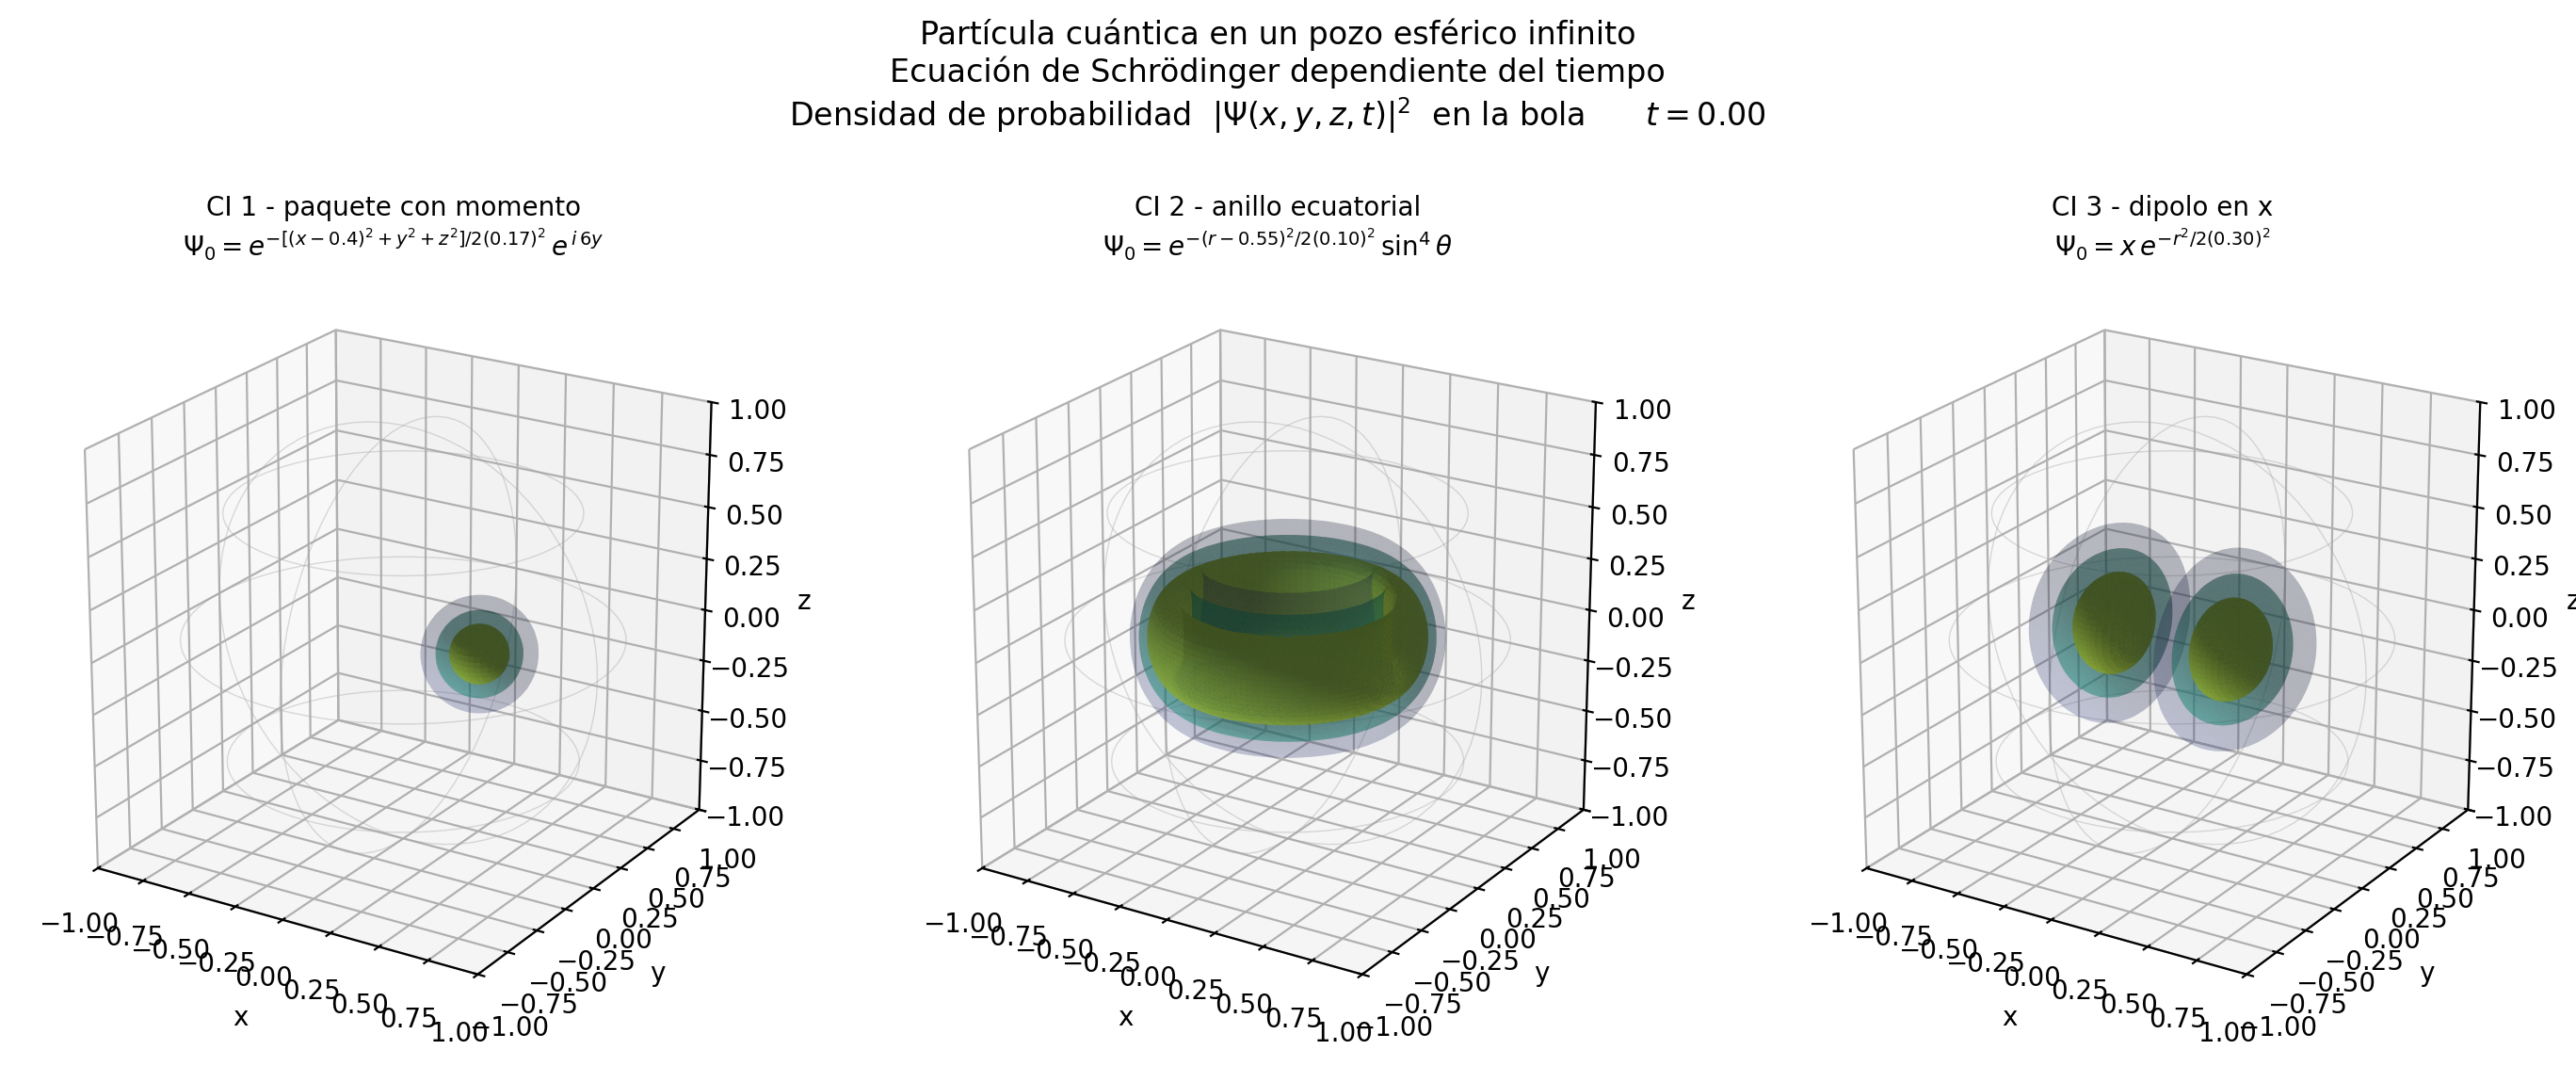
\includegraphics[width=0.98\textwidth]{frame_3d.png}
    \caption{Visualización tridimensional de la densidad de probabilidad $|\Psi(x,y,z,t)|^2$ en el instante inicial. Se comparan un paquete con momento, un anillo ecuatorial y una condición tipo dipolo en la dirección $x$.}
    \label{fig:visualizacion-3d}
\end{figure}

\begin{figure}[htbp]
    \centering
    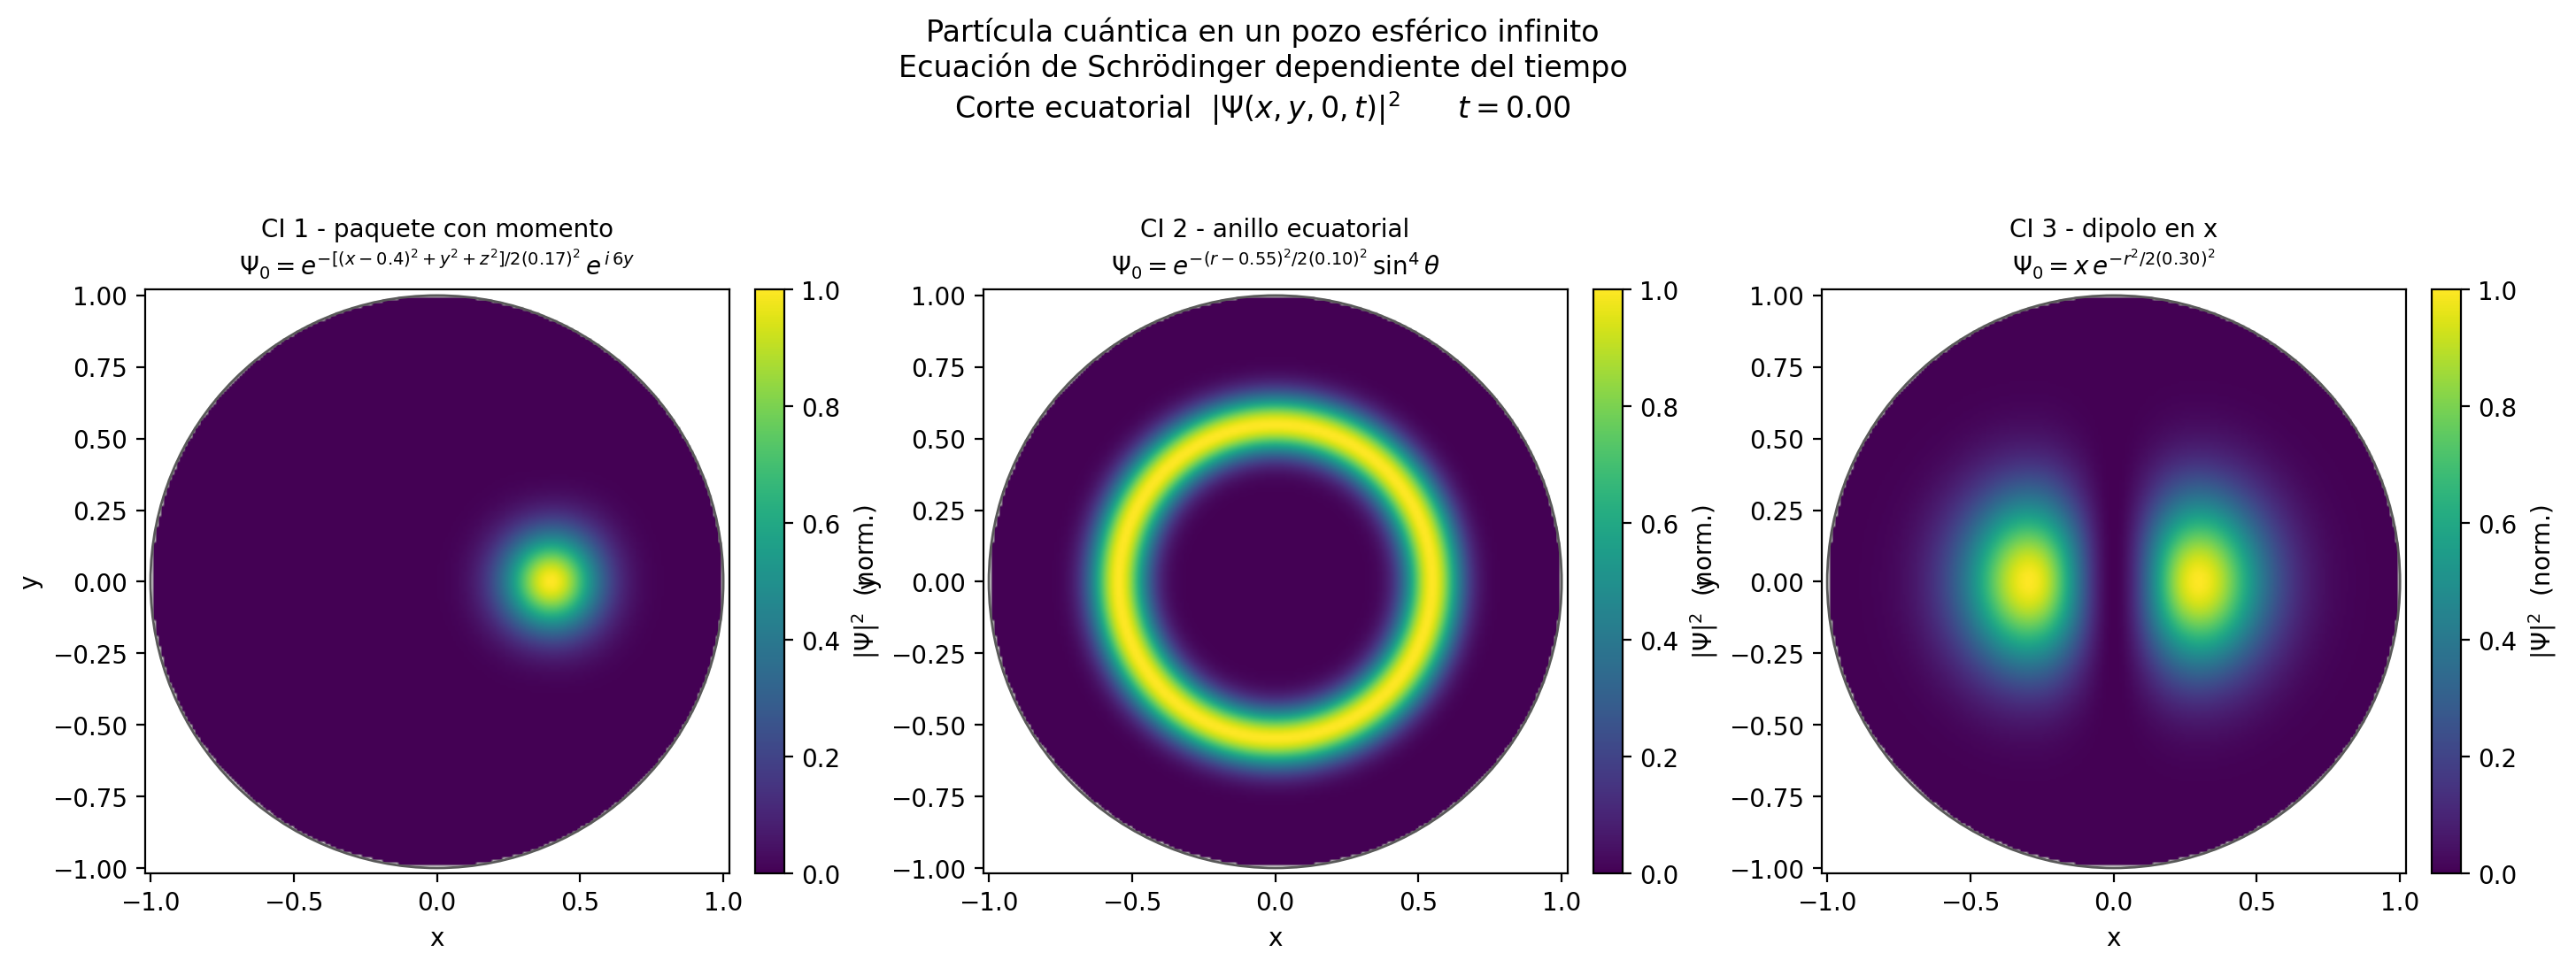
\includegraphics[width=0.98\textwidth]{frame_2d.png}
    \caption{Corte ecuatorial de la densidad de probabilidad $|\Psi(x,y,0,t)|^2$ en el instante inicial. Esta vista permite identificar con mayor claridad la localización inicial del paquete, la simetría azimutal del anillo y los dos lóbulos de la condición tipo dipolo.}
    \label{fig:visualizacion-2d}
\end{figure}

\section*{Comparación de funciones de Bessel esféricas}

Las siguientes figuras ilustran el criterio usado en la parte radial. Las funciones de segunda especie se descartan por su singularidad en el origen, mientras que las funciones modificadas no permiten satisfacer la condición de borde homogénea en $r=a$ mediante soluciones finitas y no triviales.

\begin{figure}[htbp]
    \centering
    \includesvg[width=0.88\textwidth]{bessel_esfericas_ordinarias}
    \caption{Funciones esféricas de Bessel ordinarias para $l=0,\dots,5$. Las funciones $j_l$ son regulares en el origen, mientras que las funciones $y_l$ divergen al acercarse a $x=0$.}
    \label{fig:bessel-ordinarias}
\end{figure}

\begin{figure}[htbp]
    \centering
    \includesvg[width=0.88\textwidth]{bessel_esfericas_modificadas}
    \caption{Funciones esféricas de Bessel modificadas para $l=0,\dots,5$. Las funciones $i_l$ crecen y no presentan ceros para argumento positivo; las funciones $k_l$ divergen en el origen y decrecen para argumentos grandes.}
    \label{fig:bessel-modificadas}
\end{figure}

\end{document}
